
\section{Static Network Conditions}\label{sec:static}

\begin{figure*}[]
	%\vspace{-10em}
    \begin{subfigure}[t]{0.33\textwidth}      
    		\centering
        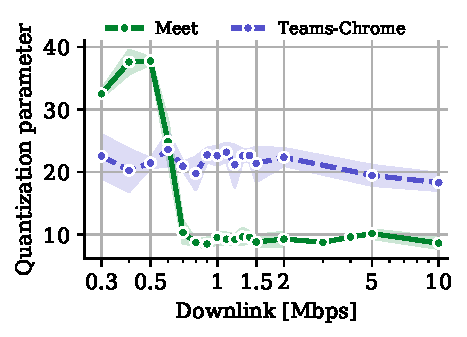
\includegraphics[width=\textwidth,keepaspectratio]{figures/static/downlink_r_qpsum.pdf}
        \caption{Downlink - Quantization parameter}
 		\label{subfig:downlink_video_qp}
    \end{subfigure}%
    \hfill
	\begin{subfigure}[t]{0.33\textwidth}   
        \centering
        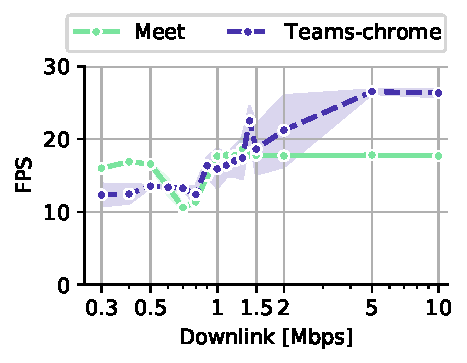
\includegraphics[width=\textwidth]{figures/static/downlink_received_framesPerSecond.pdf}
    \caption{Downlink - Frames per second}
    \label{subfig:downlink_frames_per_second}
    \end{subfigure}% 
    \hfill
	\begin{subfigure}[t]{0.33\textwidth}   
        \centering
        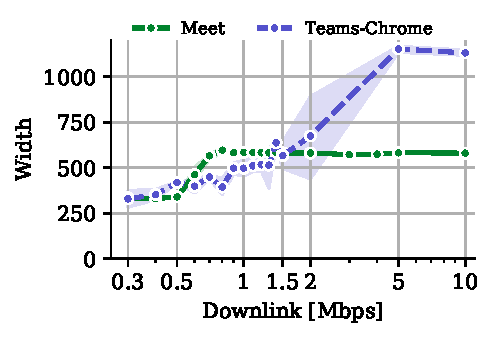
\includegraphics[width=\textwidth]{figures/static/downlink_received_frameWidth.pdf}
    \caption{Downlink - Frame width}
    \label{subfig:downlink_frame_width}
    \end{subfigure}
    \newline
        \begin{subfigure}[t]{0.33\textwidth}      
    		\centering
        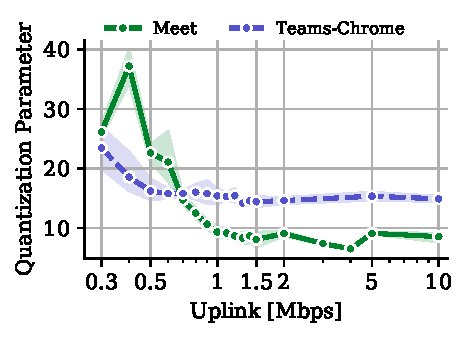
\includegraphics[width=\textwidth,keepaspectratio]{figures/static/uplink_s_qpsum.pdf}
        \caption{Uplink - Quantization parameter}
 		\label{subfig:uplink_video_qp}
    \end{subfigure}%
    \hfill
	\begin{subfigure}[t]{0.33\textwidth}   
        \centering
        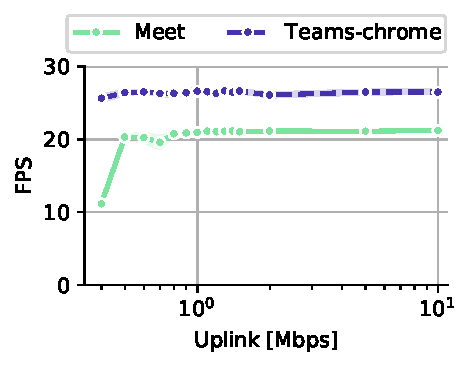
\includegraphics[width=\textwidth]{figures/static/uplink_sent_framesPerSecond.pdf}
    \caption{Uplink - Frames per second}
    \label{subfig:uplink_frames_per_second}
    \end{subfigure}% 
    \hfill
	\begin{subfigure}[t]{0.33\textwidth}   
        \centering
        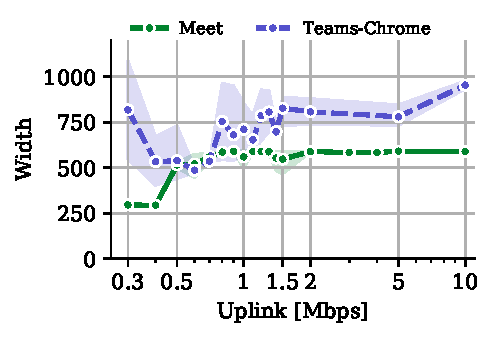
\includegraphics[width=\textwidth]{figures/static/uplink_sent_frameWidth.pdf}
    \caption{Uplink - Frame width}
    \label{subfig:uplink_frame_width}
    \end{subfigure}
	%\vspace{-1em}
	\caption{Video quality metrics under downlink and uplink shaping}
	\label{fig:video_qual}
	%\vspace{-1em}
\end{figure*}



In this section, we study the impact of network capacity on the VCA performance. Each experiment consists of a 2.5-minute call between C1 and C2 under a specific shaping level. We conduct two set of experiments with uplink shaped in the first set and downlink shaped in the second set. We consider the following shaping levels: \{$0.3, 0.4, \dots, 1.5, 2, 3, 4, 5, 10$\} Mbps with 5 repetitions at each shaping level.  We also include the browser clients for \zoom and \teams, referred to as \zoombrowser and \teamsbrowser, respectively. This is done to understand if there are any platform-related differences. 
%% experiment setup
%% what is the experiment duration 
%% what bandwidth profiles are used 

% \tarun{Open questions: i) What about Team native client? ii) Audio performance? iii) Re-do \zoombrowser for 0.3 Mbps and 0.4 Mbps}



\subsection{Network utilization}
\textbf{Uplink shaping}: Figure~\ref{subfig:uplink_bitrate} shows the median sent network bitrate at different uplink shaping levels. The bands represent the 90\% confidence intervals. We find differences in uplink network utilization among VCAs under the same network conditions. For unconstrained uplink (10 Mbps), the average uplink utilization for \teamsnative is $1.44$ Mbps whereas it is only $0.95$ for \meet and $0.77$ Mbps for \zoom. All three VCAs utilize the uplink efficiently (above 85\%) for constrained uplink (0.8 Mbps or lower) with \meet slightly better than the other VCAs.  


\textbf{Downlink shaping}: We next analyze the impact of downlink shaping on VCAs' network utilization as shown in Figure~\ref{subfig:downlink_bitrate}. Similar to uplink shaping, the VCAs differ in terms of their downlink utilization under unconstrained link. The unconstrained downlink utilization is also different from the uplink counterpart as shown in Table~\ref{tab:vca_static}. To understand this, we analyze the traffic captured on both C1 and C2. For \teams, we found that the sent traffic on C1 is almost same as the received traffic on C2 and vice versa. Thus, the differences may largely be due to the variability across runs in \teams as is also evident in the larger confidence intervals compared to \zoom and \meet. 

For \zoom, we found an asymmetry in sent and received data on both C1 and C2. For instance, in a single instance with 10 Mbps downlink shaping, C2 sent a median 0.85 Mbps and C1 received a median 1.10 Mbps. We analyze the traffic source and find that \zoom uses a relay server instead of direct communication. Related work by Nistico et al.~\cite{nistico2020comparative} alludes that \zoom uses Forward Error Correction (FEC) for error recovery. This is further supported by a related patent from \zoom itself, which talks about a methodology to generate FEC data at the server~\cite{liu2019error}. Thus, the extra data may correspond to FEC data added by the relay server leading to asymmetric uplink and downlink utilization.  

For \meet, in addition to the asymmetric unconstrained utilization, the behavior under constrained links is also markedly different. Specifically, the network utilization under constrained downlink (< 0.8 Mbps) is only 39\%-70\% (Figure~\ref{subfig:downlink_bitrate}), while it is more than $90\%$ in the case of uplink shaping (Figure~\ref{subfig:uplink_bitrate}). On digging deeper, we find that \meet also uses a relay server. In addition, it uses \textit{simulcast} wherein the sender (C2) transmits two copies of the video to the server, one at a high quality and the other at a low quality~\cite{nistico2020comparative}. The server then relays one of the stream to C1 depending on the inferred available capacity of the server-C1 link. For constrained link, the relay server still can't switch to a higher quality video and keeps sending at low quality bitrate. This explains why \meet's network utilization at 0.5 Mbps is only 0.19 Mbps, almost similar to its utilization at 0.3 Mbps.  The use of \textit{simulcast} also explains the higher uplink utilization compared to downlink. %To further validate it, we plot the utilization at 

% The network utilization of \teams is also lower during downlink shaping, compared to uplink utilization. While, it is not clear \zoom, on the other hand, uses a scalable video coding (SVC), wherein the video is encoded at multiple hierarchical layers at the sender. The server now can construct multiple versions of the video by using a subset of layers. \teams, on the other hand, uses the server as a true relay server without any congestion control at the sender. 


\textbf{Impact of device platform}: Figure~\ref{subfig:uplink_browser} compares the uplink utilization of \zoom and \teams between their native and chrome client. While, the utilization of \zoom matches on both the platforms, we find significant difference between \teams native and browser client. At 1 Mbps uplink, \teams-native client utilizes 0.84 Mbps, whereas \teamsbrowser utilizes only 0.61 Mbps. We found a similar difference between \teams-native and \teamsbrowser under downlink shaping. This suggests that VCA implementation can differ across platforms leading to different network and application behavior. 


\begin{figure}[t]
    \centering
    \begin{subfigure}[t]{0.35\textwidth}      
        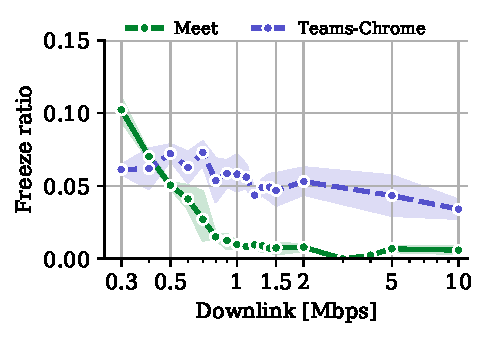
\includegraphics[width=\textwidth,keepaspectratio]{figures/static/downlink_freezeRatio.pdf}
        \caption{Downlink: Freeze ratio}
 		\label{subfig:downlink_freeze_ratio}
    \end{subfigure}
	\begin{subfigure}[t]{0.35\textwidth}   
        \centering
        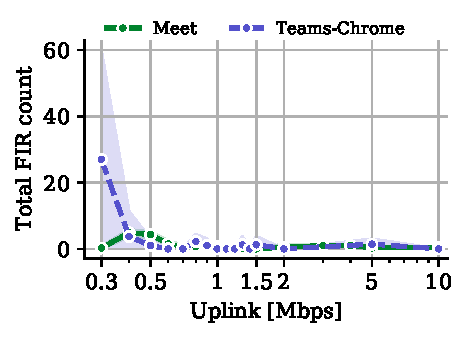
\includegraphics[width=\textwidth]{figures/static/uplink_sent_firCount.pdf}
        \vspace{-2em}
    \caption{Full Intra Request (FIR) count}
    \label{subfig:uplink_fir}
    \end{subfigure}% 
	\caption{Video freeze under downlink and uplink shaping}
	\label{fig:video_freeze}
	%\vspace{-1em}
\end{figure}


\begin{table}[]
\centering
\begin{tabular}{|c|c|c|}
\hline
\multirow{2}{*}{\textbf{VCA}} & \multicolumn{2}{c|}{\textbf{Utilization {[}Mbps{]}}} \\ \cline{2-3} 
                              & Uplink                   & Downlink                  \\ \hline
Meet                          & 0.95                     & 0.84                      \\ \hline
Teams                         & 1.40                      & 1.86                      \\ \hline
Zoom                          & 0.78                     & 0.95                      \\ \hline
\end{tabular}
\caption{Unconstrained network utilization}
\label{tab:vca_static}
\end{table}



%We next analyze the median sent network bitrate for different uplink capacity (see Figure~\ref{fig:uplink_bitrate}). As expected, we find similar differences in terms of the maximum bitrate among the VCAs and between browser and native clients for \teams as observed in the downlink shaping experiment. However, the network utilization is higher, especially for \meet, when the upstream link is constrained as compared to downlink. Thus, there seems to be a discrepancy in bitrate adaptation when the upstream is constrained. We explore this discrepancy in more detail in Section~\ref{sec:interruption}. 

\subsection{Application performance}
Here we describe how the link shaping level impacts application performance metrics. %However, obtaining application metrics can be challenging for VCAs. 
We rely on the WebRTC stats API available in Google Chrome to obtain application metrics for \teamsbrowser and \meet~\cite{webrtc_stats}. We could not obtain the same statistics for \zoombrowser as it uses DataChannels instead of RTP MediaStream API in WebRTC to transmit media. Video quality statistics are not exposed for DataChannels. Obtaining application metrics is challenging for native clients.  % We could not obtain the same statistics for \zoombrowser as it used different transport channels to transmit media, i.e., datachannels instead of the RTP MediaStream~\cite{webrtc_stats} as it may provides more flexibility (e.g., flexible encoding standards) to \zoom. However, video quality statistics are not exposed anymore through the WebRTC stats API. %In addition, we also obtained access to Zoom API through our campus network operator. The Zoom API provides limited application performance (e.g., video resolution, FPS) at a per-minute granularity~\cite{zoom_qos_api}. 
Thus, we limit this analysis to only \meet and \teamsbrowser. We focus on a subset of metrics available from WebRTC Stats API that relate to video \textit{quality} and \textit{freezes}. These metrics are available at a per-second granularity within the call. % The metrics are described in the We consider only a subset of metrics 

%More specifically, we consider the following application metrics: Frames per second, video resolution, freeze ratio. 

\textbf{Video quality}: VCAs adapt the video quality by adjusting the encoding parameters to achieve a target bitrate estimate provided by the transport. Ideally, VCAs can adjust one or more of the following three parameters: i) frames per second (\textit{FPS}), ii) \textit{quantization parameter} used in video compression, and  iii) \textit{video resolution} indicating the number of pixels in each dimension. We can obtain all three parameters from the WebRTC stats. In our analysis, we indicate resolution with one of the dimension, i.e., the \textit{frame width}. 

We first look at these parameters for different downlink shaping levels (see~\Cref{subfig:downlink_video_qp,subfig:downlink_frames_per_second,subfig:downlink_frame_width}). We find that \teamsbrowser simultaneously degrades all three parameters as the downlink becomes more constrained. There is also significant variance across multiple repetitions under the same network bandwidth as shown by the $90\%$ confidence interval bands in the plot. \meet, on the other hand, follows a more consistent trend where it adjusts parameters differently based on the shaping level. Within 0.7-1 Mbps region, the bitrate is controlled mostly by adapting the \textit{FPS} while keeping the \textit{quantization parameter} and \textit{frame width} similar to the nominal levels. However, going from 0.7 to 0.5 Mbps, both \textit{frame width} and \textit{quantization parameter} degrade whereas there is an increase in the FPS. From a closer inspection of the per-second statistics within this region, we find that the relay server starts switching to the lower quality copy of the stream it received via \textit{simulcast}. \meet does not seem to reduce the bitrate any further by reducing the FPS for the low quality stream indicated by consistent FPS below 0.5 Mbps. It is not clear why the quantization parameter reduces from 38 to 33 at 0.3 Mbps in \meet. 

We next analyze the impact of uplink shaping on encoding parameters (see~\Cref{subfig:uplink_video_qp,subfig:uplink_frames_per_second,subfig:uplink_frame_width}). We find that \teams adapts to the shaping level mainly by increasing the quantization parameter and reducing the frame width, while keeping the FPS almost constant. The frame width, surprisingly, increases at 0.3 Mbps uplink shaping level. This may be an artifact of a poor design decision as we find that it leads to frame losses (see next paragraph). \meet follows a similar trend by mostly increasing the quantization parameter until the uplink bandwidth degrades to 0.5 Mbps. At 0.4 Mbps, it also reduces frame width and the FPS. 

\textbf{Video Freezes}: We also analyze the statistics related to video freezes. For downlink shaping, we directly obtain the freeze duration from WebRTC stats wherein a freeze is assumed to occur if the frame inter-arrival $>$ max (3$\delta$, $\delta$ + $150 ms$). $\delta$ is the average frame duration. We normalize the freeze duration with the call duration to obtain freeze ratio.  Figure~\ref{subfig:downlink_freeze_ratio} show the freeze ratio under different downlink shaping levels. Freeze ratio increases as the downlink bandwidth degrades. The freezes are more severe in \meet than \teamsbrowser with $10\%$ freeze ratio at 0.3 Mbps. Interestingly, \teamsbrowser incurs some freezes ($3.6\%$) even under unconstrained links. 

For uplink shaping, we could not obtain freeze statistics directly as logging is done at C1. Instead, we analyze the total count of Full Intra Requests (FIR) during a session. An FIR is sent if the receiver cannot decode the video or falls behind, likely due to frame losses. Note that a low FIR count does not rule out freezes on the receiver but a high count does indicate issues. Figure~\ref{subfig:uplink_fir} shows that the FIR count is particularly high for \teamsbrowser at uplink capacity below 0.5 Mbps. A high FIR count in \teamsbrowser may be triggered due to the sender sending high resolution video (see Figure~\ref{subfig:uplink_frame_width})


% \textbf{Takeaway}: Uplink 

\textbf{Takeaway}: VCA performance under same network conditions varies among tested VCAs. Further, the minimum bandwidth requirements have implications for broadband policy. The FCC currently recommends a 25/3 Mbps minimum connection. Such a connection would not suffice for two separate video conferences. A household with a parent working and a child attending class remotely would saturate the uplink and lead to poor user experience. 
%% also plot differences in network utilization and the shaping. 



%% Difference among VCAs. Peak utlization differs. For the same network conditions, VCAs peform differently. For instance, Teams on WebRTC 
%% Difference between native and browser client 
%% Google Meet Simulcast




